\documentclass[11pt,a4paper]{article}

\usepackage[margin=2.4cm]{geometry}
\usepackage{newtxtext}
\usepackage{microtype}
\usepackage{setspace}
\usepackage{booktabs}
\usepackage{graphicx}
\usepackage{caption}
\usepackage{xcolor}
\usepackage{tikz}
\usetikzlibrary{arrows.meta,positioning}
\usepackage{enumitem}
\usepackage{hyperref}
\usepackage{fancyhdr}
\usepackage{titlesec}

\hypersetup{colorlinks=true,linkcolor=black,urlcolor=black}
\definecolor{phaseblue}{HTML}{2F5496}
\definecolor{donegreen}{HTML}{2E6B4A}
\definecolor{latergray}{HTML}{666666}

\pagestyle{fancy}
\fancyhf{}
\fancyhead[L]{\small WAPDA Maintenance Cost Project}
\fancyhead[R]{\small Project Walkthrough}
\fancyfoot[C]{\thepage}
\renewcommand{\headrulewidth}{0.3pt}

\titleformat{\section}{\large\bfseries\color{phaseblue}}{\thesection.}{0.5em}{}
\titleformat{\subsection}{\normalsize\bfseries}{\thesubsection}{0.4em}{}
\setlist[itemize]{leftmargin=1.2em,itemsep=0.22em}
\setlist[enumerate]{leftmargin=1.3em,itemsep=0.22em}
\setlength{\parskip}{0.35em}
\setlength{\parindent}{1em}

\begin{document}

\begin{center}
{\large\bfseries\color{phaseblue} WAPDA Staff-Colony Maintenance Cost Prediction}\\[0.4em]
{\LARGE\bfseries What We Did and Why}\\[0.5em]
{\large A plain-language record of the full project journey}\\[0.6em]
{\normalsize Saeed Ahmad \textperiodcentered{} CAIP Batch 8 \textperiodcentered{} August 2026}\\[0.3em]
{\small From data assessment to model comparison and Phase~2 improvements}
\end{center}

\vspace{0.5em}
\noindent\rule{\textwidth}{0.5pt}

\section*{Purpose of this document}
This document is not the short CAIP exam report. It is a longer explanation for anyone who wants to understand the whole project: what problem we chose, what data we had, what we built, which models we tried, and why we made each major decision.

The project belongs to the WAPDA staff-colony maintenance planning idea. The work was done carefully so that results are honest, repeatable, and safe to explain to managers without overstating what the numbers prove.

\section{The problem we wanted to solve}

WAPDA maintains houses and apartments in staff colonies. Each year, maintenance money must be planned for civil work, plumbing, electrical repairs, roofing, painting, sewerage, and emergency fixes.

Today, budgets often rely on:
\begin{itemize}
  \item past averages across many houses,
  \item manual inspections,
  \item complaint lists,
  \item engineering judgement.
\end{itemize}

That works at a rough level, but it treats very different properties as if they were the same. An old bungalow with repeated plumbing problems is not the same as a recently repaired flat, yet both may receive the same average allowance.

\textbf{Our goal:} for one house or apartment, estimate eligible maintenance cost for the \textbf{next twelve months}, and also flag properties that are likely to become \textbf{high-cost} cases.

\textbf{Two jobs, not one:}
\begin{enumerate}
  \item \textbf{Budget number} --- how much will this property cost next year?
  \item \textbf{Priority list} --- which properties deserve early attention?
\end{enumerate}

The original proposal also planned a web application where a user could pick a property and see the estimate. That application is still future work. This project completed the data and modelling foundation.

\section{What we found in the WAPDA / WASC files}

We started with real WAPDA-related material in the \texttt{DatasetOfCAIP/} folder:
\begin{itemize}
  \item occupancy and inventory lists for \textbf{101 residential units} (categories A--F),
  \item property presentations and land/asset documents,
  \item a repair-and-maintenance ledger with hundreds of transactions.
\end{itemize}

These files were valuable. They defined the \textbf{real WAPDA problem}: 101 in-scope residential units, eligible maintenance types, shared-building cost sharing, and privacy rules.

But they were \textbf{not enough} to train a property-level machine learning model because:
\begin{itemize}
  \item the ledger is mostly \textbf{account-level}, not cleanly linked to one house and one work order,
  \item many charges cannot be tied to a completed job on a specific property,
  \item names, CNIC, salaries, and free-text remarks must stay private,
  \item linked WAPDA work-order and invoice extracts were \textbf{not released} for training under current privacy rules.
\end{itemize}

\textbf{Important rule we kept:} a missing ledger line is \textbf{not} the same as zero cost. Zero is only valid when coverage proves that no eligible work happened.

\textbf{Decision:} keep WASC files as private \textbf{seed evidence} for scope and policy, and build a separate \textbf{public training dataset} mapped to the same WAPDA data model.

\section{The WAPDA data model we fixed first}

Before any modelling, we wrote down exactly what one training row means in WAPDA terms:

\begin{table}[ht]
\centering
\caption{The WAPDA data model (the rulebook for every row).}
\begin{tabular}{@{}lp{10cm}@{}}
\toprule
Element & Meaning \\
\midrule
One row & One residential property on one cutoff date \\
Target & Eligible maintenance cost for the next 12 months \\
Included & Routine, corrective, emergency building work + fair share of shared building cost \\
Excluded & Major renovation, rebuilding, appliances, land, rent, revenue entries \\
Scope & 101 WASC residential units only (not offices, roads, mosque, hospital, etc.) \\
High-cost flag & Top 20\% of costs in the training fold \\
Features & Only facts known on or before the cutoff date \\
\bottomrule
\end{tabular}
\end{table}

This model came from WAPDA/WASC framing. The training table was then \textbf{filled} using public housing survey data that could be mapped to these fields. That is why we say the dataset is \textbf{made on the WAPDA data model}, even though the dollar amounts come from a U.S.\ survey proxy, not from WAPDA invoices.

\section{Phase 1 --- Dataset preparation}

Phase~1 was about building a clean, honest dataset and making sure the evaluation could not cheat.

\subsection{Step 1: Register and validate sources}

We registered every source file with hashes and version information so nothing could change silently. Raw WASC files stayed untouched. Public sources (RHFS and AHS) were validated for integrity before use.

\textbf{Why:} reproducibility and trust. If someone asks ``where did this number come from?'', we can point to a registered file and a transformation log.

\subsection{Step 2: Two public dataset slices (kept separate)}

We built two real public slices, but \textbf{never mixed their labels}:

\begin{table}[ht]
\centering
\caption{Public training slices (separate tasks).}
\begin{tabular}{@{}llrr@{}}
\toprule
Release & What it is & Properties & Labels \\
\midrule
RHFS 2024 & Cross-sectional U.S.\ rental properties & 4,425 & 1,488 annual repair labels \\
AHS 2015--2023 & Longitudinal U.S.\ housing survey & 36,623 linked units & 86,125 pairs \\
\bottomrule
\end{tabular}
\end{table}

\textbf{RHFS} was useful as an early slice and proof of the pipeline. \textbf{AHS} became the main modelling corpus because it supports \textbf{time-based} learning: we see a house in one survey year and its maintenance cost in the next survey wave (two years later).

The AHS gate passed because we had far more than the 500-property minimum (36,623 units).

\textbf{Why AHS for the main experiments:} maintenance forecasting needs history and a future label on the same house. AHS gives linked before/after pairs. RHFS is a different kind of label and stays a separate experiment view.

\subsection{Step 3: Map survey fields onto the WAPDA model}

Example mappings:
\begin{itemize}
  \item building type \texttt{BLD} $\rightarrow$ WAPDA building type,
  \item year built \texttt{YRBUILT} $\rightarrow$ property age,
  \item rooms and bedrooms $\rightarrow$ size proxies,
  \item earlier \texttt{MAINTAMT} $\rightarrow$ past maintenance cost (feature),
  \item later \texttt{MAINTAMT} $\rightarrow$ future maintenance cost (target).
\end{itemize}

\textbf{Why mapping matters:} the model learns WAPDA-shaped inputs, not random survey columns. When WAPDA operational data becomes available later, the same field names and rules can be reused.

\subsection{Step 4: Split the data without leakage}

We used a \textbf{grouped temporal split}. Each house belongs to only one of training, validation, or test. The same house never teaches the model and also appears in the final exam.

\begin{table}[ht]
\centering
\caption{AHS split (\texttt{ahs-grouped-temporal-v1}).}
\begin{tabular}{@{}lrrl@{}}
\toprule
Set & Houses & Rows & Used for \\
\midrule
Training & 10,103 & 13,871 & Learn cleaning rules and fit models \\
Validation & 7,067 & 15,400 & Choose settings (pick lowest MAE) \\
Test & 19,453 & 56,854 & Final score only \\
\bottomrule
\end{tabular}
\end{table}

We also kept a second test view that \textbf{removes 2023 labels}, because the 2023 survey changed its maximum reportable maintenance amount. That sensitivity check stops us from confusing a survey rule change with model skill.

\textbf{Why this split design:} random row splits would let the same house appear in both training and testing. That would inflate scores and mislead decision-makers.

\subsection{Step 5: Preprocessing (training data only)}

On training rows only, we learned:
\begin{itemize}
  \item how to fill missing numeric values (medians),
  \item how to encode categories,
  \item the high-cost cutoff (USD~1,428 = top 20\% of training costs).
\end{itemize}

Then we applied those rules to validation and test without looking at their labels for learning.

The first feature matrix had \textbf{205 columns}. The target was never changed, imputed, or clipped.

\textbf{Why training-only preprocessing:} if validation or test labels influence cleaning rules, the model is graded on data it already saw. That is a common source of hidden cheating in machine learning projects.

\section{Phase 1 --- First model comparison (Experiment 1)}

Once the dataset was ready, we ran a fixed, documented comparison: \texttt{ahs-baselines-models-v1}.

\subsection{What we compared}

\textbf{Simple baselines} (easy to explain to a manager):
\begin{itemize}
  \item \textbf{Training median} --- predict the middle cost seen in training,
  \item \textbf{Type median} --- predict the middle cost for that building type,
  \item \textbf{Prior cost} --- predict last period's maintenance cost.
\end{itemize}

\textbf{Learning models} (from the proposal):
\begin{itemize}
  \item Linear regression,
  \item Random Forest,
  \item Gradient boosting.
\end{itemize}

\textbf{Why include baselines:} a complex model must beat a simple, transparent rule. If it cannot, there is no reason to deploy it.

\subsection{How we measured success (in plain words)}

\begin{itemize}
  \item \textbf{MAE} --- average dollar error. Lower is better. Main score for picking models.
  \item \textbf{RMSE} --- like MAE, but large mistakes hurt more.
  \item \textbf{High-cost F1} --- how well we find expensive houses (above USD~1,428). Higher is better.
\end{itemize}

\subsection{Main Phase~1 results (primary test set)}

\begin{table}[ht]
\centering
\caption{Experiment 1 --- key test-set scores (USD).}
\begin{tabular}{@{}lrrr@{}}
\toprule
System & Test MAE & Test RMSE & High-cost F1 \\
\midrule
Type median & 962.81 & 2361.65 & --- \\
Prior cost & 1058.25 & 2358.81 & \textbf{0.410} \\
Linear regression & 950.91 & 2182.90 & 0.384 \\
Random Forest & 956.54 & 2188.13 & 0.397 \\
Gradient boosting & \textbf{949.15} & 2188.68 & 0.356 \\
\bottomrule
\end{tabular}
\end{table}

\textbf{What this showed:}
\begin{itemize}
  \item Gradient boosting had the \textbf{lowest test MAE} among fitted models.
  \item Type median was still best on the \textbf{validation} set (827.95 USD), which is the score we chose models by.
  \item Prior cost was best at finding \textbf{high-cost} houses (F1 = 0.410).
  \item Improvements were real but small --- tens of dollars on errors that are already hundreds of dollars.
\end{itemize}

\subsection{The selection policy (why we did not declare a ``winning AI model'')}

We wrote a rule \textbf{before} looking at excuses after the test:
\begin{enumerate}
  \item Pick by \textbf{validation MAE}, not test MAE.
  \item Also report the no-2023 sensitivity test and high-cost F1.
  \item Promote a fitted model only if it wins validation \textbf{and} is at least as good on the sensitivity test.
\end{enumerate}

Under that rule:
\begin{itemize}
  \item \textbf{Official cost estimator:} type median,
  \item \textbf{Official high-cost reference:} prior cost,
  \item \textbf{Promoted fitted model:} none.
\end{itemize}

\textbf{Why this matters:} it stops us from chasing a small test-set win that may not survive a rule change or a new data year. It also matches public-sector needs: a simple rule people can audit often beats a black box by a few dollars.

\section{Experiment 2 --- Log1p target transform (tried and rejected)}

\textbf{What we did:} train the same models on $\log(1 + \text{cost})$ instead of raw dollars, then convert predictions back to dollars for scoring.

\textbf{Why we tried it:} maintenance costs are skewed (many small, few very large). Log transforms often help tree models with heavy tails.

\textbf{What happened:} average error sometimes looked slightly better on validation, but \textbf{high-cost detection collapsed}. On the test set, gradient boosting F1 fell from 0.356 to 0.008.

\textbf{Decision:} do not use log1p training as the reporting path. The problem was not mainly ``wrong scale''; feature quality and model settings mattered more.

\section{Phase 2 --- Model improvement sequence}

After Experiment~1 and the log1p check, we opened a structured Phase~2 plan (\texttt{Documentation/next\_steps.md}). The order was deliberate: \textbf{understand features before heavy tuning}.

\begin{figure}[ht]
\centering
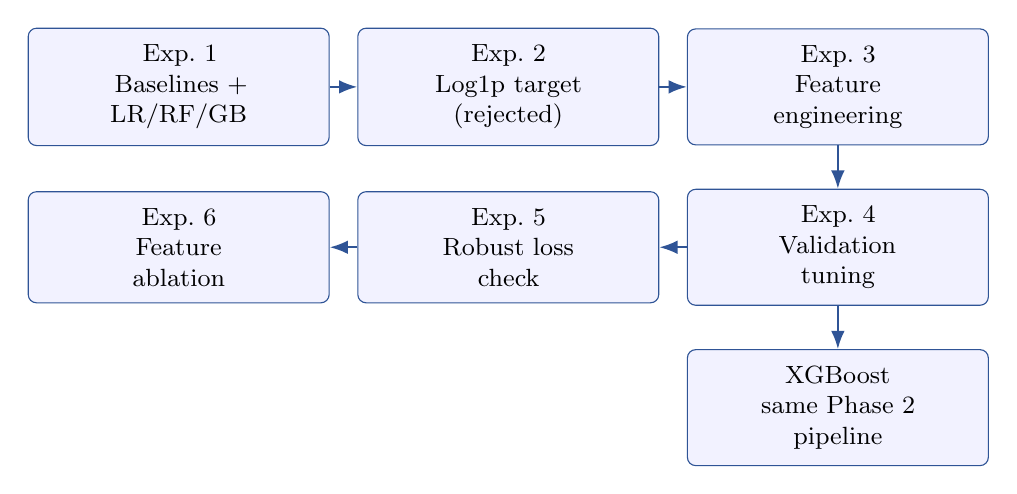
\begin{tikzpicture}[
  font=\small,
  flowstep/.style={draw=phaseblue, fill=blue!5, rounded corners=3pt, align=center,
               inner sep=6pt, text width=3.4cm, minimum height=1.1cm},
  arr/.style={-{Latex}, thick, phaseblue}
]
\node[flowstep] (e1) {Exp.\ 1\\Baselines + LR/RF/GB};
\node[flowstep, right=0.35cm of e1] (e2) {Exp.\ 2\\Log1p target\\(rejected)};
\node[flowstep, right=0.35cm of e2] (e3) {Exp.\ 3\\Feature\\engineering};
\node[flowstep, below=0.55cm of e3] (e4) {Exp.\ 4\\Validation\\tuning};
\node[flowstep, left=0.35cm of e4] (e5) {Exp.\ 5\\Robust loss\\check};
\node[flowstep, left=0.35cm of e5] (e6) {Exp.\ 6\\Feature\\ablation};
\node[flowstep, below=0.55cm of e4] (xg) {XGBoost\\same Phase~2\\pipeline};
\draw[arr] (e1) -- (e2);
\draw[arr] (e2) -- (e3);
\draw[arr] (e3) -- (e4);
\draw[arr] (e4) -- (e5);
\draw[arr] (e5) -- (e6);
\draw[arr] (e4) -- (xg);
\end{tikzpicture}
\caption{Phase~2 experiment sequence. Feature engineering came before tuning on purpose.}
\end{figure}

\subsection{Phase 2, Step 1 --- Feature audit}

\textbf{What we did:} reviewed all 205 model columns on 13,871 training rows.

\textbf{Why:} tuning a weak feature set wastes time. We needed to know what was missing, redundant, or unsuitable.

\textbf{Findings:}
\begin{itemize}
  \item 26 harmonized survey fields expanded to 205 encoded columns,
  \item roof leak field had very high missingness (kept missing flag, dropped unreliable values),
  \item no continuous floor-area field (so ``cost per sqft'' was not directly available),
  \item survey weight is for survey design, not for WAPDA operations.
\end{itemize}

\subsection{Phase 2, Step 2 --- Feature engineering (Experiment 3)}

We added five simple derived features that are easier for models to use:
\begin{itemize}
  \item property age = survey year minus year built,
  \item log of past maintenance cost,
  \item past cost divided by number of rooms,
  \item rooms per bedroom,
  \item count of condition/defect flags.
\end{itemize}

The matrix grew from 205 to \textbf{215 columns}. Preprocessing audits passed.

\textbf{Result alone:} small change on primary test MAE (gradient boosting 949.15 $\rightarrow$ 950.42). Engineering by itself was not a magic fix, but it prepared better inputs for tuning.

\textbf{Why still worth doing:} derived features match how engineers think (age, burden, intensity), and they unlock gains when combined with tuning.

\subsection{Phase 2, Step 3 --- Preprocessing check}

We confirmed both preprocessors (original and engineered) learn only from training data. Linear regression uses standardized numeric inputs; tree models use the same encoded matrix.

\textbf{Why:} different models must still follow the same leakage-safe contract.

\subsection{Phase 2, Step 4 --- Validation-only tuning (Experiment 4)}

\textbf{What we did:} search hyperparameters for Random Forest and gradient boosting on the \textbf{validation set only}, then refit the best settings on training data. Linear regression settings stayed fixed.

\textbf{Why validation-only:} the test set must remain a true final exam. Tuning on test data would be another form of cheating.

\textbf{Primary test MAE after tuning:}
\begin{itemize}
  \item Random Forest: 956.54 $\rightarrow$ \textbf{946.57}
  \item Gradient boosting: 949.15 $\rightarrow$ \textbf{945.27}
\end{itemize}

Tuning helped tree models by about 4--10 USD on average error --- modest but real.

\subsection{Phase 2, Step 5 --- Robust loss comparison (Experiment 5)}

\textbf{What we did:} compare squared error vs absolute error vs Huber loss for gradient boosting.

\textbf{Why:} absolute error focuses on typical misses and can ignore expensive outliers --- we needed to see if that trade was acceptable.

\textbf{Result:}
\begin{itemize}
  \item Absolute loss: test MAE \textbf{899.84} (best MAE in this sequence),
  \item But high-cost F1 fell to \textbf{0.065} (almost stops finding expensive houses),
  \item Squared loss kept better balance for prioritisation.
\end{itemize}

\textbf{Lesson:} a lower average error can be the wrong goal if the organisation also needs a priority list.

\subsection{Phase 2, Step 6 --- Inflation sensitivity (deferred)}

We documented a plan but did not run it as a main experiment because the 2023 survey cap change already dominates nominal-dollar drift. A separate inflation adjustment would not cleanly separate ``price inflation'' from ``survey rule change''.

\subsection{Phase 2, Step 7 --- Feature ablation (Experiment 6)}

\textbf{What we did:} train gradient boosting with different feature groups removed.

\textbf{Why:} tell WAPDA which information actually drives forecasts.

\textbf{Key result:} removing past maintenance features raised test MAE from 947.79 to \textbf{979.67} (about USD~32 worse).

\textbf{Actionable conclusion:} a future WAPDA system needs reliable \textbf{property-level maintenance history}. Building characteristics alone are not enough.

\subsection{Phase 2 extension --- XGBoost pipeline}

The proposal mentioned advanced tree models; we added XGBoost on the same engineered features and Phase~2 steps:
\begin{itemize}
  \item XGBoost with fixed settings,
  \item validation-only tuning (144 combinations),
  \item absolute-error objective check (same MAE vs F1 tradeoff as gradient boosting).
\end{itemize}

\textbf{Best balanced fitted model on the full test set:} tuned XGBoost --- MAE \textbf{944.34}, RMSE \textbf{2182.07}, high-cost F1 \textbf{0.391}.

\textbf{Why XGBoost:} strong industry default for tabular data; good check that Phase~2 gains were not specific to one sklearn implementation.

\section{Software, tests, and governance (why the work is trustworthy)}

We did not only train models in notebooks. The project is a Python package (\texttt{caip\_maintenance}) with:
\begin{itemize}
  \item config files for splits, preprocessors, and experiments,
  \item command-line steps for harmonize, split, preprocess, train, and audit,
  \item automated tests for leakage, metric math, and artifact reload,
  \item privacy rules: no PII in tests, logs, or reports; raw WASC files stay local.
\end{itemize}

\textbf{Why this extra work:} CAIP requires real implementation, not just slides. WAPDA would also need auditable pipelines before any operational use.

\section{What we can say confidently today}

\begin{table}[ht]
\centering
\caption{Plain-language summary of outcomes.}
\begin{tabular}{@{}p{4.2cm}p{9.8cm}@{}}
\toprule
Topic & Conclusion \\
\midrule
Dataset & Built on the WAPDA data model; filled with mapped AHS public data because WAPDA work orders were unavailable \\
Best simple budget rule & Type median (validation MAE 827.95 USD) \\
Best simple priority rule & Prior cost (high-cost F1 0.410) \\
Best tuned learning model & XGBoost (test MAE 944.34; F1 0.391) \\
Absolute-error models & Lower MAE but poor at finding expensive houses --- not suitable alone for prioritisation \\
Past maintenance history & Strongly important (ablation + prior-cost results) \\
WAPDA operational forecast & \textbf{Not validated yet} --- needs linked WAPDA costs in PKR \\
Web application & Planned; not built in this phase \\
\bottomrule
\end{tabular}
\end{table}

\section{What remains for a full WAPDA deployment}

\begin{enumerate}
  \item \textbf{Operational WAPDA data} --- anonymized property IDs, dated work orders, verified costs, shared-building allocations, and explicit coverage rules.
  \item \textbf{PKR labels} --- the current proxy is in U.S.\ survey dollars.
  \item \textbf{Web proof of concept} --- property lookup, estimate display, high-cost list, colony summaries.
  \item \textbf{Pilot on selected colonies} --- compare predictions to actual outcomes after data access is approved.
  \item \textbf{Monitoring} --- detect when survey or accounting rule changes break model assumptions (we already saw this risk with the 2023 AHS cap).
\end{enumerate}

\section{Timeline in one view}

\begin{table}[ht]
\centering
\caption{Major project stages (simplified timeline).}
\small
\begin{tabular}{@{}llp{7.8cm}@{}}
\toprule
Stage & Status & What happened \\
\midrule
Problem \& proposal & Done & WAPDA maintenance cost + prioritisation; CAIP scope \\
WASC data assessment & Done & 101-unit inventory; ledger not property-linked enough \\
Dataset policy & Done & Public multi-source training path approved \\
RHFS release & Done & First public slice; pipeline proof \\
AHS release & Done & Main corpus: 86,125 linked pairs \\
Split \& preprocess & Done & Grouped temporal split; training-only fit \\
Experiment 1 & Done & Baselines + LR/RF/GB; selection policy applied \\
Experiment 2 & Done & Log1p target rejected \\
Phase 2 steps 1--7 & Done & Audit, engineering, tuning, robust loss, ablation \\
XGBoost Phase 2 & Done & Tuned XGBoost best balanced learner \\
CAIP report \& code annex & Done & PDF report, zip annex, test source file \\
Web POC & Later & Not started \\
WAPDA validation & Blocked & Waiting on operational extracts \\
\bottomrule
\end{tabular}
\end{table}

\section{Closing note}

This project did real work on a real public-sector problem under real privacy limits. It did not pretend that survey dollars are WAPDA invoices. It built the WAPDA-shaped data model, tested simple rules before complex models, wrote the selection rules in advance, and ran a full Phase~2 improvement path when the first experiments showed that target transforms alone were not the answer.

The most useful message for WAPDA is practical: \textbf{start collecting property-linked maintenance history now}. The models confirm that past spending and building type carry much of the signal. When operational data arrives, the same workflow --- split by time, train safely, compare against simple baselines, report honestly --- is ready to use.

\vspace{0.5em}
\noindent\rule{\textwidth}{0.4pt}\\
{\small Related files: \texttt{reports/submission/caip\_final\_report.pdf} (exam report),
\texttt{Documentation/AHSNextStepsExecution.md} (Phase~2 log),
\texttt{Documentation/DatasetPolicy.md} (data strategy).}

\end{document}
